\documentclass{article}
\usepackage{amsmath,amsfonts,amsthm, amssymb, mathtools} % Math packages
\setlength\parindent{0pt} % Removes all indentation from paragraphs - comment this line for an assignment with lots of text
\usepackage{graphicx}
\newcommand\SetSymbol[1][]{\:#1\vert\:}
\providecommand\given{} % to make it exist
\DeclarePairedDelimiterX\Set[1]\{\}{\renewcommand\given{\SetSymbol[\delimsize]}#1}
\DeclareMathOperator{\lcm}{lcm}
\usepackage{color}
\usepackage{listings}

\definecolor{dkgreen}{rgb}{0,0.6,0}
\definecolor{gray}{rgb}{0.5,0.5,0.5}
\definecolor{mauve}{rgb}{0.58,0,0.82}

\lstset{frame=tb,
  language=Python,
  aboveskip=3mm,
  belowskip=3mm,
  showstringspaces=false,
  columns=flexible,
  basicstyle={\small\ttfamily},
  numbers=none,
  numberstyle=\tiny\color{gray},
  keywordstyle=\color{blue},
  commentstyle=\color{dkgreen},
  stringstyle=\color{mauve},
  breaklines=true,
  breakatwhitespace=true,
  numbers=left,
  tabsize=3
}

\begin{document}
\title{Written Assignment \#2}
\author{Ben Haines (bmh5wx)}

\section*{Problem \# 1}
Problem Description: Return the set of sleeping points that minimizes the number of stops needed for a given trip.\\

Inputs:
\begin{itemize}
    \item $L$ = length of the trip.
    \item $d$ = maximum distance that can be traveled in one day.
    \item stops = list $(x_1, x_2, \ldots, x_n)$ of locations of stopping points.
\end{itemize}

Outputs: List of locations from input list indicating where to stop for the night.\\

Assumptions:
\begin{itemize}
    \item The distance between every two successive stops is less than or equal to $d$.
    \item A perfect ability to determine whether or not you can make it to the next stop in time.
    \item Inputs are finite.
\end{itemize}

Strategy Overview:
I will use a greedy algorithm that travels the maximum possible distance on any given day.\\

Algorithm Description:
\begin{lstlisting}
define getStops(L, d, stops):
    output = []
    total = 0
    for i in range(len(stops)):
        if L - total <= d:
            return  output
        elif stops[i] - total <= d and (i+1 >= len(stops) or stops[i+1] - total > d):
            output.append(stops[i])
            total = stops[i]

    return output
\end{lstlisting}

\section*{Problem \# 2}
I want to show that the greedy algorithm produces an optimal solution. First I'll prove a lemma that the greedy solution always "stays ahead." Let $O(o_1, o_2, \ldots, \o_n)$ be the set of stopping points selected by the optimal algorithm. Let $G = (g_1, g_2, \ldots, g_m)$ be the set of stopping points selected by the greedy algorithm. By the definition of optimal, $n \le m$. \\

\underline{Lemma:} $\forall_{1\le i\le m} g_i \ge o_i$. \\

That is, the $i^{th}$ greedy stopping point is always at least as far along as the $i^{th}$ optimal stopping point. I'll prove this lemma by induction.\\

Base Case: $i=1$. WTS: $g_1 \ge o_1$. This is done by simple contradiction. If $o_1$ was farther along than $g_1$ the greedy solution would have chosen it by definition.\\

Inductive Hypothesis: Assume $\forall_{1\le i\le k-1} g_o \ge o_i$ for some $k\ge 1$. \\

Inductive Step: WTS that $g_k \ge o_k$. Assume that $g_k < o_k$. Then by the inductive hypothesis $o_k - g_{k-1} < g_k - g_{k-1}$ and $o_k - o_{k-1} \ge g_k - g_{k-1}$. These inequalities mean that the greedy solution didn't select the point $o_k$ even though it was reachable from $g_{k-1}$ and farther along than the point that was selected. This is a contradiction so $g_k \ge o_k$ and the lemma is proved.\\

Finally I want to show that $|O|=|G|$. $|O| = n$ and $|G| = m$ so assume that $n < m$. The optimal solution contains $n$ stops which means that $L$ was reachable from stop $o_n$ and thus $L - o_n \le d$. By the lemma proven above, $L - g_n \le d$ which means that $L$ is reachable from the $n^{th}$ stop in the greedy solution. This implies $n=m$ which is a contradiction. Thus $|O| = |G|$.

\section*{Problem \#3}
Problem Description: Find the shortest path between two cities given variable travel times along different roads.\\

Inputs:
\begin{itemize}
    \item $G$ = graph representing various paths.
    \item $s$ = start node
    \item $t$ = end node
    \item $f(u, v, t)$ = function that returns end time after traveling from node $u$ to node $v$ at start time $t$
\end{itemize}

Outputs: Shortest path between $s$ and $t$.\\

Assumptions:
\begin{itemize}
    \item You can't travel backwards in time.
    \item You will never arrive earlier by leaving later.
    \item There is only one edge between two vertices.
    \item The graph is connected.
\end{itemize}

Strategy Overview:
The solution is essentially identical to Dijkstra's shortest path algorithm. In this case we are given a specific cost function.\\

Algorithm Description:
\begin{lstlisting}
Vertex[] Graph::dijkstra(Vertex s, Vertex t):
  Vertex v,w
  for node in Graph: 
    node.dist = infinity
  s.dist = 0;

  while (there exist unknown vertices, find the 
        unknown Vertex v with the smallest distance)
    v.known = true;

    for each w adjacent to v
      if (!w.known)
          if (v.dist + f(v, w, v.dist) < w.dist):
          w.dist = v.dist + f(v, w, v.dist);
          w.path = v;
        
  Vertex current = t;
  Vertex[] finalPath = [t]
  while (current.path != none):
      finalPath.append(current.path)
      current = current.path

  return finalPath

\end{lstlisting}

The running time of the algorithm depends on the specifics of the implementation. Under the given assumptions it's possible to implement this algorithm such that it has a running time of $O(ElogV)$ where $E$ is the number of edges in the graph and $V$ is the number of vertices in the graph.

\section*{Problem \#4}
We want to prove that the distance calculated by Dijkstra to each node is minimal. We express this as:
$$\forall_i dist(S_i)\text{ is minimal}$$
We do this by induction on $i$. The base case is trivial because the algorithm sets the minimum distance of the start node $S_0$ to 0 which is also the minimum distance. Thus, the base case is proven.\\
\textbf{Inductive Hypothesis:} Assume that for some $k$, $\forall_{i\le k}dist(S_i)$ is minimal.\\
\textbf{Inductive Step:} Show that $dist(S_{k+1})$ is minimal.\\

We do this in the following way. We know the algorithm makes the following calculation for $dist(S_{k+1})$:
$$dist(S_{k+1}) = \min(dist(S_i) + f(S_i, S_{k+1}, dist(S_i))\text{Where }i\le k$$

Remember that we know that all $S_i$ distances are minimal if $i\le k$ by the inductive hypothesis. We also know that the choice the algorithm made is better than all other equivalent minimum distances plus one extra edge to an unknown node. We prove that this is the best possible distance to $S_{k+1}$ by contradiction.\\

Assume for the sake of contradiction that:
$$dist(S_i) + f(S_i, S_{k+1}, dist(S_i))\text{ not minimal}$$
Then it follows, with $\delta > 0$. 
$$\exists_{j\not= i}|dist(S_j) + f(S_j, S_{k+1}, dist(S_i)) + \delta < dist(S_i) + f(S_i, S_{k+1}, dist(S_i))$$
In the best case $\delta = 0$ so 
        $$dist(S_j) + f(S_j, S_{k+1}, dist(S_j)) < dist(S_i) + f(S_i, S_{k+1}, dist(S_i))$$
This is a contradiction because it indicates the algorithm didn't choose what it is defined to choose. Thus the algorithm always calculates the minimum distance between two nodes. The given algorithm simply records what vertexes are used when finding the minimum distance and thus the returned path is trivially the shortest path between the two points.

\section*{Problem \#5}
\begin{enumerate}
    \item Every MST of $G$ is an Elite Tree of $G$.\\
        Prove by contraposition. Assume that $T$ is some spanning tree of $G$ that is not elite. Let $e_1$ be the maximum edge in $T$. Edge $e_1$ connects two subtrees $A$ and $B$ of $T$. It is given that $T$ is not an elite tree and thus there must be some other edge $e_2$ that also connects $A$ and $B$ but which has a lower weight than $e_1$. Replacing $e_1$ with $e_2$ in $T$ produces a spanning tree with weight less than $T$ thus $T$ is not an MST.

        By contraposition, this proves that every MST of a graph $G$ is an Elite Tree of $G$.

    \item It is not the case that every Elite Tree of $G$ is an MST of $G$. In the following image (next page) the green edges form an elite tree that is not an MST.
    \begin{figure}[hb]
        \centering
        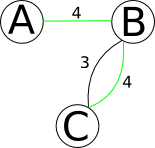
\includegraphics[scale=0.5]{eliteNotMST}
    \end{figure}
\end{enumerate}
\end{document}
